\documentclass[12pt,a4paper]{../krautsourcing/homework}
\usepackage[utf8]{inputenc}
\usepackage[ngerman]{babel}
\usepackage[T1]{fontenc}
\usepackage{amsmath}
\usepackage{graphicx}
\usepackage{amsfonts}
\usepackage{amssymb}
\usepackage{lmodern}
\usepackage{amsmath}
\usepackage{amssymb}
\usepackage{paralist}
\usepackage{tabularx}
\usepackage{tikz}
\usetikzlibrary{automata,positioning,backgrounds}

\author{Ruben Felgenhauer,\\Alexander Hildebrandt,\\Leonhard Reichenbach}
\datef{03}{01}{2016}
%\date{\today}
\course{Formale Grundlagen der Informatik II}
\sheet{10}
\sectionprefix{Übungsaufgabe \thesheet.}
\subsectionprefix{\thesheet.}
\subsubsectioncounter{\alph{subsubsection}}
\group{06}
\subsubsectionprefix{(}
\subsubsectionsuffix{)}

\begin{document}

\makeheadline

\addtocounter{section}{2}

\section{}

\subsection{}

Die Wirkungsmatrix von \(N_{10.3}\) ist gegeben durch:
\begin{align*}
	\Delta = \left( \begin{array}{c|ccccc}
		& a & b & c & d & e \\
		\hline
		p1 & -1 & -1 & 4 & 2 & -3\\
		p2 & 0 & -1 & 4 & 0 & 0\\
		p3 & 0 & 1 & -4 & 0 & 0\\
		p4 & 1 & 2 & -8 & -2 & 3\\
	\end{array} \right)
\end{align*}
Somit ist die Menge aller T-Invarianten: \(J = \{(-3x+2y,4z,z,y,x)^T \mid x,y,z \in \mathbb{N}\}\)

\subsection{}

\newcommand{\cvec}[1]{\begin{pmatrix}#1\end{pmatrix}}

Wir wählen die \(\mathbf{m_0} = (4,4,0,0,0)^T\) und die Schaltfolge \(w = bbbbceadd\):
\begin{align*}
    \cvec{4\\4\\0\\0}
    \xrightarrow{b}
    \cvec{3\\3\\1\\2}
    \xrightarrow{b}
    \cvec{2\\2\\2\\4}
    \xrightarrow{b}
    \cvec{1\\1\\3\\6}
    \xrightarrow{b}
    \cvec{0\\0\\4\\8}
    \xrightarrow{c}
    \cvec{4\\4\\0\\0}
    \xrightarrow{e}
    \cvec{1\\4\\0\\3}
    \xrightarrow{a}
    \cvec{0\\4\\0\\4}
    \xrightarrow{d}
    \cvec{2\\4\\0\\2}
    \xrightarrow{d}
    \cvec{4\\4\\0\\0}
\end{align*}
Offensichtlich ist \(\Psi(w) = (1,4,1,2,1)\).

\section{}

\subsection{}

Die gegebenen Transformationsregeln verändern die Korrektheit eines Workflow-Netzes nicht. Zudem können wir jedes korrekte Netz soweit vergröbern, bis wir ein triviales Netz erhalten. Gelingt die Transformation mit den gegebenen Regeln, ist das Netz also korrekt. Somit können wir mit diesen Regeln die Korrektheit eines Workflow-Netzes untersuchen. \(\hfill \square\)

\subsection{}

Das kleinste korrekte Workflow-Netz besteht nur aus einer Stelle und es gilt \(a = e\).

\subsection{}

\newcommand{\raisetop}[1]{\raisebox{\dimexpr-\totalheight\relax}{#1}}

\Huge\bfseries
\resizebox{\textwidth}{!}{
\begin{tabular}{lc}
\hline
0: & \raisetop{{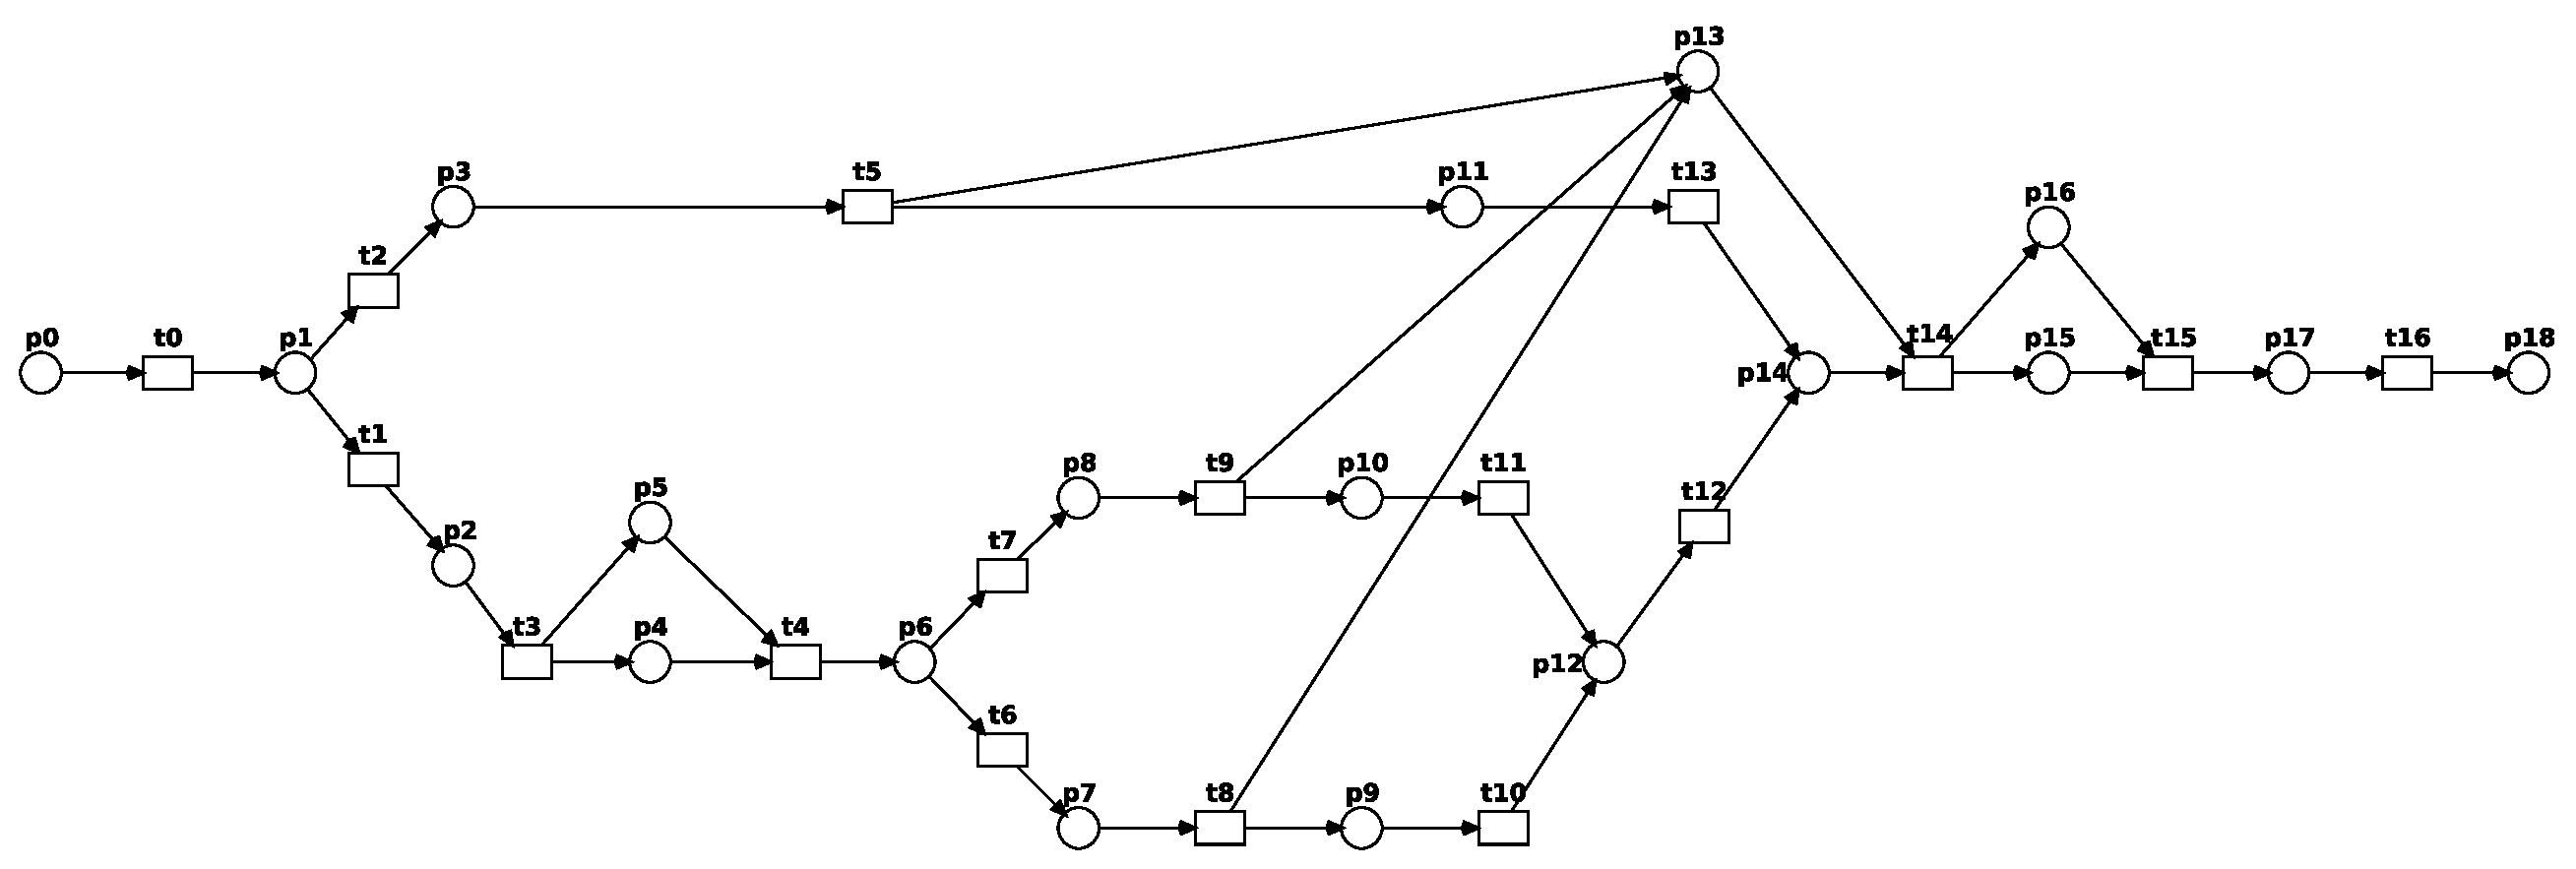
\includegraphics{aufgabe-10-4-3/aufgabe-10-4-3__0.pdf}}} \\
\hline
1: & \raisetop{{\includegraphics{aufgabe-10-4-3/aufgabe-10-4-3__1.pdf}}} \\
\hline
2: & \raisetop{{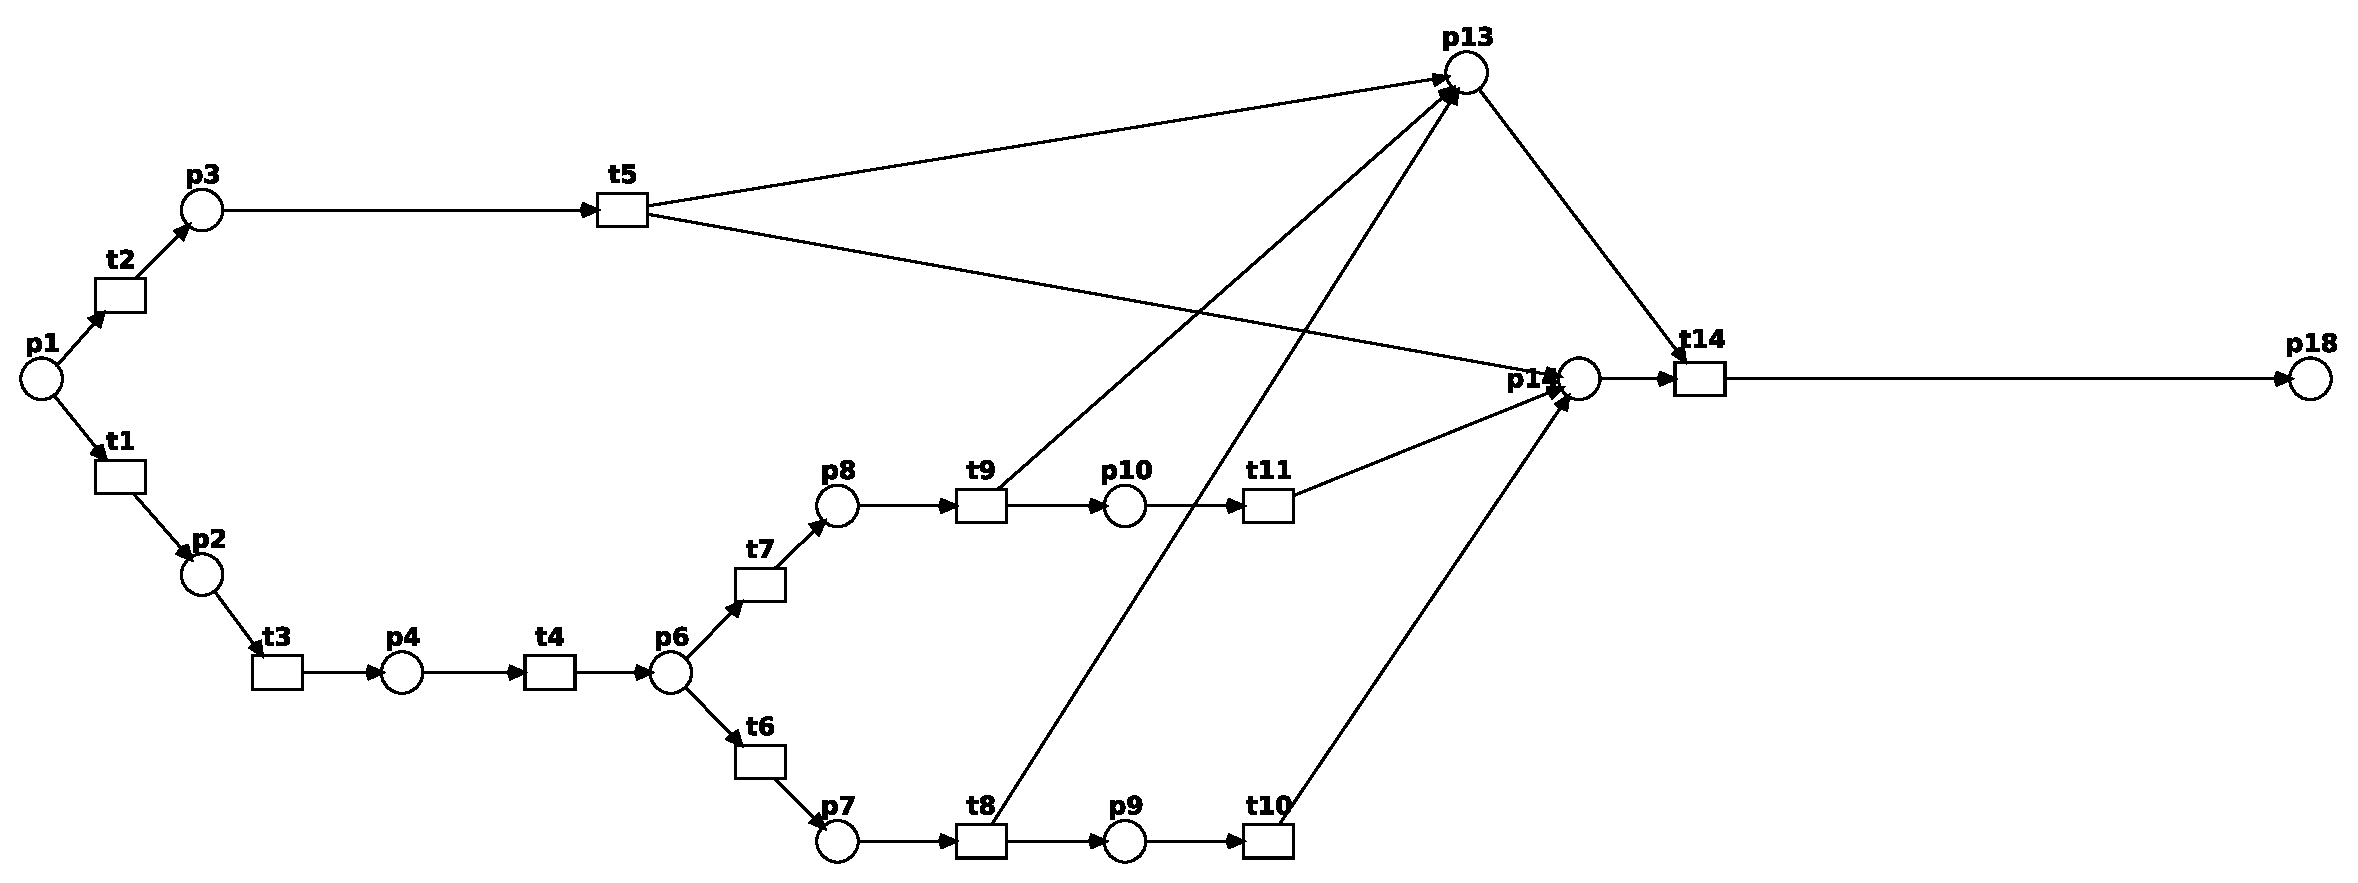
\includegraphics{aufgabe-10-4-3/aufgabe-10-4-3__2.pdf}}} \\
\hline
3: & \raisetop{{\includegraphics{aufgabe-10-4-3/aufgabe-10-4-3__3.pdf}}} \\
\end{tabular}
}
\newpage
\resizebox{\textwidth}{!}{
\begin{tabular}{lc}
4: & \raisetop{{\includegraphics{aufgabe-10-4-3/aufgabe-10-4-3__4.pdf}}} \\
\hline
5: & \raisetop{{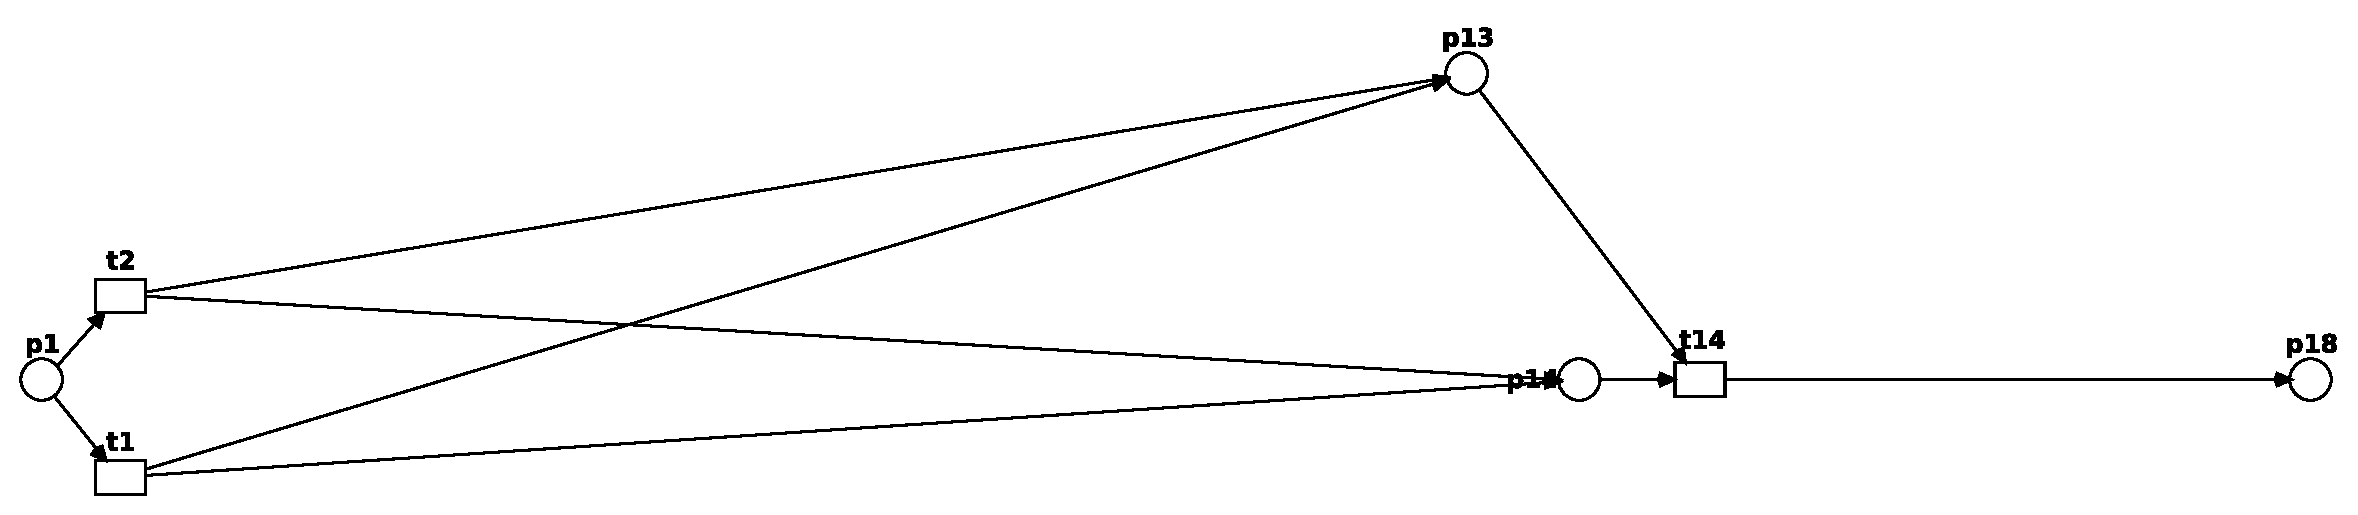
\includegraphics{aufgabe-10-4-3/aufgabe-10-4-3__5.pdf}}} \\
\hline
6: & \raisetop{{\includegraphics{aufgabe-10-4-3/aufgabe-10-4-3__6.pdf}}} \\
\hline
7: & \raisetop{{\includegraphics{aufgabe-10-4-3/aufgabe-10-4-3__7.pdf}}} \\
\hline
8: & \raisetop{{
\includegraphics{aufgabe-10-4-3/aufgabe-10-4-3__8.pdf}}} \\
\end{tabular}
}
\normalsize\normalfont

\subsection{}

\def\tabularxcolumn#1{m{#1}}
\centerline{
\begin{tabularx}{\textwidth}{|*2{c|} *2{>{\centering\arraybackslash}X|}}
\hline
Nr. & Transformationsregel & Verbliebene Knoten & Entfernte Knoten\\
\hline
0 & Originalnetz & p0, ..., p18, t0, ..., t16 & - \\
\hline
1 & Par & p0, ..., p4, p6, ..., p15, p17, p18, t0, ..., t16 & p5, p16 \\
\hline
2 & P-Seq & p1, ..., p4, p6, ..., p10, p13, p14, p18, t1, ..., t11, t14 & p0, p11, p12, p15, p17, t0, t12, t13, t15, t16 \\
\hline
3 & T-Seq & p1, p6, p13, p14, p18, t1, t2, t6, t7, t14 & p2, p3, p4, p7, ..., p10, t3, t4, t5, t8, ..., t11 \\
\hline
4 & Same Pre/Post & p1, p6, p13, p14, p18, t1, t2, t6, t14 & p6, t7 \\
\hline
5 & T-Seq& p1, p13, p14, p18, t1, t2, t14 & t6  \\
\hline
6 & Same Pre/Post & p1, p13, p14, p18, t1, t14 & t2 \\
\hline
7 & Par & p1, p13, p18, t1, t14 & p14 \\
\hline
8 & P-Seq & p18 & p1, p13, t1, t14 \\
\hline
\end{tabularx}
}

\vspace*{10mm}

\subsection{}

Der zusätzliche Zustand \gqq{px} erfordert eine Regel wie \gqq{Same Pre/Post}, die für Stellen statt für Transitionen gilt. Da wir so eine Regel nicht gegeben haben, können wir das Netz nicht vollständig vergröbern.

\subsection{}

Wir betrachten den Erreichbarkeitsgraphen des Netzes:\\
\centerline{
\begin{tikzpicture}[auto,baseline,node distance=15mm]
    \node                      (p4)   {\(p4\)};
    \node[right=of p4]         (p6px) {\(p6,px\)};
    \node[below right=of p6px] (p7px) {\(p7,px\)};
    \node[above right=of p6px] (p8px) {\(p8,px\)};
    \node[right=of p7px]       (p9)   {\(p9\)};
    \node[right=of p8px]       (p10)  {\(p10\)};
    \node[below right=of p10]  (p12)  {\(p12\)};
    %
    \path[->,shorten <=1mm, shorten >=1mm]
        (p4)   edge node[above]       {\(t4\)}  (p6px)
        (p6px) edge node[below left]  {\(t6\)}  (p7px)
        (p6px) edge node[above left]  {\(t7\)}  (p8px)
        (p7px) edge node[below]       {\(t8\)}  (p9)
        (p8px) edge node[above]       {\(t9\)}  (p10)
        (p9)   edge node[below right] {\(t10\)} (p12)
        (p10)  edge node[above right] {\(t11\)} (p12)
    ; %-path-%
\end{tikzpicture}
}
\begin{compactenum}[\bfseries a)]
\item Offensichtlich führt jede mögliche Schaltfolge letztendlich zum Endplatz \(e = p12\), also ist aus jeder erreichbaren Markierung eine ordnungsgemäße Terminierung möglich.
\item Die einzige Möglichkeit zu terminieren ist mit \(\mathbf{m}(p12) = 1\).
\item Wir können jede Transition \(t4,t6 \hdots, t11\) im Erreichbarkeitsgraphen wiederfinden, also ist jede Transition nützlich.
\end{compactenum}
Somit ist das gegebene Netz korrekt. \(\hfill \square\)

\subsection{}

Eine Stelle, die die selben Vor- und Nachbedingungen hat wie eine andere Stelle, kann entfernt (oder hinzugefügt) werden.

\subsection{}

Betrachten wir ein Petrinetz \(\mathcal{N}\) mit einer Teilmenge der Transitionen \(\tau \subseteq T_\mathcal{N}\), die alle den selben Vorbereich \(\Pi_V \subseteq P_\mathcal{N}\) und Nachbereich \(\Pi_N \subseteq P_{\mathcal{N}}\) besitzen. Ist \(\mathcal{N}\) beschränkt, so gilt für jede Schaltfolge, dass die Menge der Marken im Netz beschränkt ist. Umgekehrt gilt für ein unbeschränktes Netz, dass es mindestens eine Transition \(t\) gibt, bei der \(W(\bullet,t) < W(t,\bullet)\) gilt, also brutto Marken erzeugt werden. \\
Nun gilt auch, dass jedes \(t \in \tau\) exakt die gleiche Menge der Marken aus \(\Pi_V\) entfernt und ebenfalls exakt die gleiche Menge an Marken zu \(\Pi_N\) hinzufügt. Somit können wir also in jeder Schaltfolge, die ein Element aus \(\tau\) enthält, dieses \(t\) durch ein beliebiges anderes Element aus \(\tau\) ersetzen, ohne dass sich das Verhalten des Netzes ändert. Aufgrund dieser Eigenschaft können wir also auch beliebige Elemente aus \(\tau\) entfernen, solange danach \(|\tau| \geq 1\) gilt.\\
Somit verändert die Regel \textit{Same Pre/Post} die Beschränktheits-Eigenschaften eines Netzes nicht.

\(\hfill \square\)



\end{document}